

\section{Paper Summary}

\begin{figure*}
    \centering
    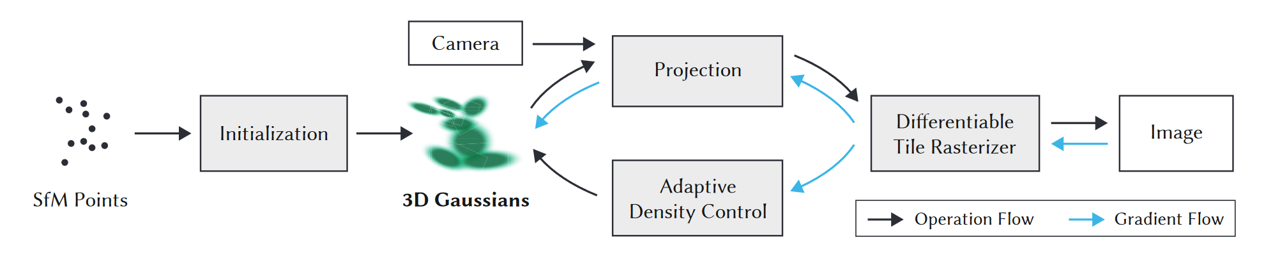
\includegraphics[width=\textwidth]{images/pipeline.png}
    \caption{The Gaussian splatting pipeline presented in the paper \cite[Fig. 2]{kerbl3DGaussianSplatting2023}.}
\end{figure*}


\subsection{Representation}
The core idea of the paper is to represent the scene as a set of Gaussians.
Each Gaussian is defined by its position $\bm{p}$, its covariance matrix $\bm{\Sigma}$, its color $\bm{c}$ and its opacity $\alpha$.

As the covariance has to be symmetric and positive definite, it is defined as
\begin{align}
    \bm{\Sigma} = \bm{R} \bm{S} \bm{S}^T \bm{R}^T,
\end{align}
where $\bm{R}$ is a rotation matrix stored as a quaternion $\bm{q}$ and $\bm{S}$ is a diagonal matrix containing the standard deviation of the Gaussian along each axis stored as a vector $\bm{s}$
To ensure that the covariance is positive definite, the diagonal elements of $\bm{S}$ are passed through a sigmoid function.
The quaternion $\bm{q}$ is normalized to ensure a proper rotation matrix.

% Similarly to other \cite{yuPlenoxelsRadianceFields2021a}\cite{mullerInstantNeuralGraphics2022}


\subsubsection{Spherical Harmonics}
\begin{figure}
    \centering
    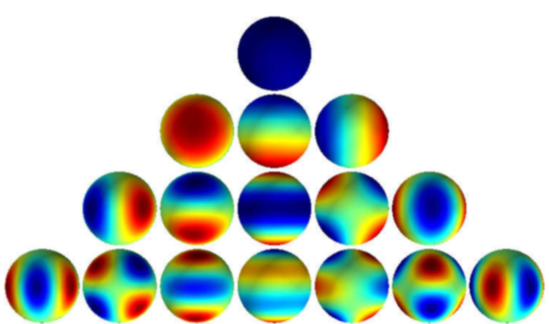
\includegraphics[width=\linewidth]{images/spherical_harmonics.png}
    \caption{Visualization of the spherical harmonics used to represent the view-dependent color of each Gaussian \cite[Fig. 3]{kerbl3DGaussianSplatting2023}.}
\end{figure}

\subsubsection{Camera Projection}

\subsection{Rasterization Pipeline}
\begin{figure}
    \centering
    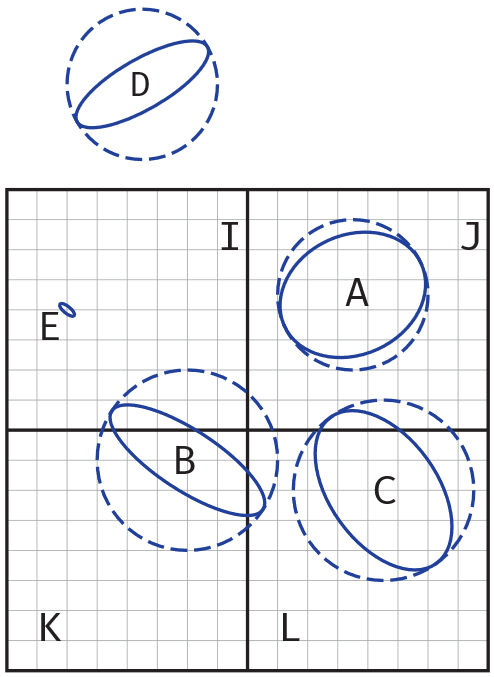
\includegraphics[width=0.6\linewidth]{images/rendering.png}
    \caption{Visualization of how Gaussian splats are rendered using multiple independent blocks.}
\end{figure}
\label{sec:rasterization}

\subsection{Densification}
\begin{figure}
    \centering
    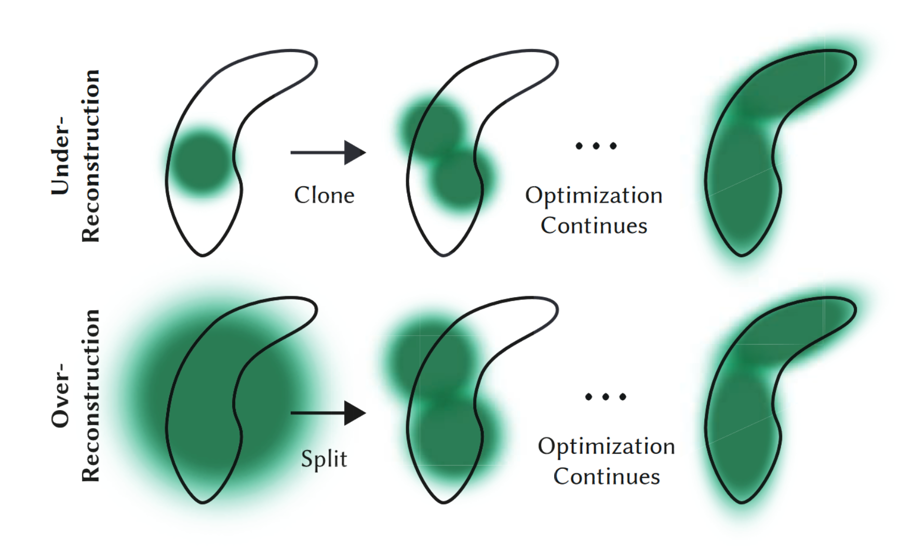
\includegraphics[width=\linewidth]{images/densification.png}
    \caption{The adaptive Gaussian densification scheme presented in the paper \cite[Fig. 4]{kerbl3DGaussianSplatting2023}.}
\end{figure}
